\section{PART II}

\begin{frame}
	\frametitle{\Large{\rm PART II}}

\begin{center}
	{\LARGE{ \bf Dissipation}\\}
	\medskip
	\medskip
	\medskip
	\texttt{ \Large
  A. Franchi, FT PR B \textbf{108}, 094114 (2023) }
\end{center}
\end{frame}

\section{Dissipation}
	\subsection{Lindblad framework}

\begin{frame}
	\frametitle{Lindblad framework}
\ba{eqlindblad}
        \frac{d\rho}{dt} = {\cal L}[\rho] =
                -i \Bigr[ H, \rho \Bigr] + \mathbb{D}[\rho] \pc
\ea

${\cal L}$ is the Liouville superoperator, and $\mathbb{D}$ is the 
dissipation term with coupling $w$:
\ba{dissipator}
        \mathbb{D}[\rho] = & w \sum_{x \in {\cal I}}
                \mathbb{D}_x[\rho] \cm \\
        \mathbb{D}_x[\rho] = &
                \hat L_x \rho \hat L_x^\dagger -
                \frac{1}{2} \Bigl\{ \rho, \hat L^\dagger_x \hat L_x \Bigl\} \pc
\ea
	

\end{frame}


\begin{frame}
\frametitle{Sunburst geometry}

\begin{figure}
    \centering
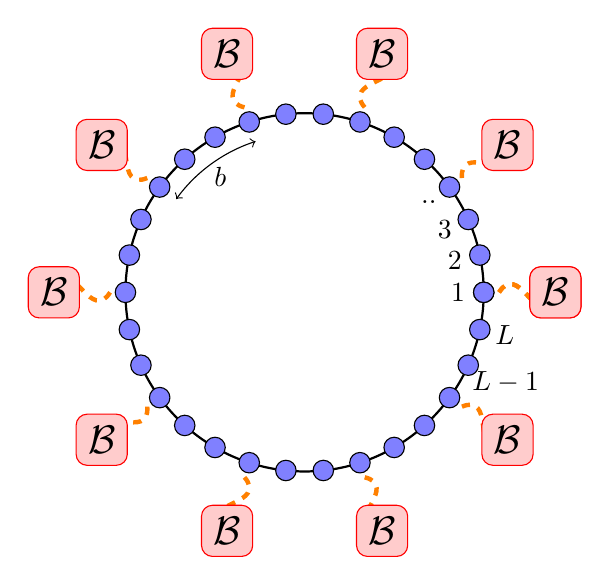
\begin{tikzpicture}[scale=0.65]
    \draw[thick] (0,0) circle (3.5cm);

    \foreach \x in {0,12,...,360}
    \filldraw [fill=blue!50] (\x:3.5cm) circle (0.2);

    \foreach \x in {0,36,...,360}
    \draw[orange, dashed, ultra thick] (\x:3.8cm) .. controls (\x+8:4.2cm) and (\x-8:4.6cm) .. (\x:4.6cm);

    \foreach \x in {0,36,...,360}
    \node[rectangle,
    draw = red,
    text = black,
    fill = red!20!white,
    rounded corners,
    minimum size=0.65cm] (r) at (\x:4.9cm) {\Large $\mathcal{B}$};

    \draw[<->] (108:3.1cm) arc
    [start angle=108,
        end angle=144,
        radius=3.1cm,
    ] ;

    \node[] (s1) at (126:2.8cm) {$b$};

    \node[] (s1) at (0:3cm) {$1$};
    \node[] (s2) at (12:3cm) {$2$};
    \node[] (s3) at (24:3cm) {$3$};
    \node[] (s4) at (36:3cm) {$..$};
    \node[] (s5) at (-12:4cm) {$L$};
    \node[] (s6) at (-24:4.3cm) {$L-1$};
\end{tikzpicture}
    \caption{Sketch of a Kitaev ring with $L=30$ qubits coupled with $n=10$ dissipators in a \textit{sunburst} geometry ($b=3$ in the figure).}
    \label{fig_sketch_sunburst_dissipation}
\end{figure}


\end{frame}


\begin{frame}
	\frametitle{Liouvillian gap}

\ba{eigencalL}
        \widetilde{\cal L}[\widetilde \rho_i] = \lambda_i \widetilde \rho_i \cm
        \qquad \lambda_i \in \numberset{C} \pc
\ea

\be{vecrho}
        \rho_{ij} \ket i \bra j  \longrightarrow  \widetilde \rho_{ij} \ket i \ket j \pt
\ee

\ba{vecteqlindblad}
        \widetilde{\mathcal{L}} =& -i \big(\hat{H} \otimes \hat{\mathbb{I}}
                - \hat{\mathbb{I}}\otimes \hat{H}^t \big) +
                w\sum_{x \in {\cal I}}\hat{L}_{x}\otimes \hat{L}^*_{x}\\
        &-\frac{w}{2}\sum_{x \in {\cal I}}\big(\hat{L}^{\dagger}_{x}\hat{L}_{x}
                \otimes\hat{\mathbb{I}}+\hat{\mathbb{I}}
                        \otimes\hat{L}^t_{x}\hat{L}^*_{x}\big) \pt
\ea

\ba{Lioulliangap}
\Delta_{\lambda} = - \max_{i} {\rm Re}{\lambda_i } \pt
\ea


\end{frame}


\begin{frame}
	\frametitle{Interplay between local and homogeneous dissipation}
	The number of the external baths:
	\be{}
		n \equiv L / b \pc
	\ee
	$ $\\
	\vspace{0.5cm}
	$b$ fixed  $\longrightarrow$ local dissipation with 
	$\Delta_\lambda \sim L^{-1} f(\mu, wL) 
	\qquad L\to\infty \pc$\\
	\vspace{1cm}
	$n$ fixed $\longrightarrow$ homogeneous dissipation with
	$\Delta_\lambda \sim L^{-3} \tilde{f}(\mu, w)
	\qquad L\to\infty\,\,$.
\end{frame}

\begin{frame}
	\frametitle{Liouvillian gap $b$ fixed}
\begin{figure}[!h]
    \centering
    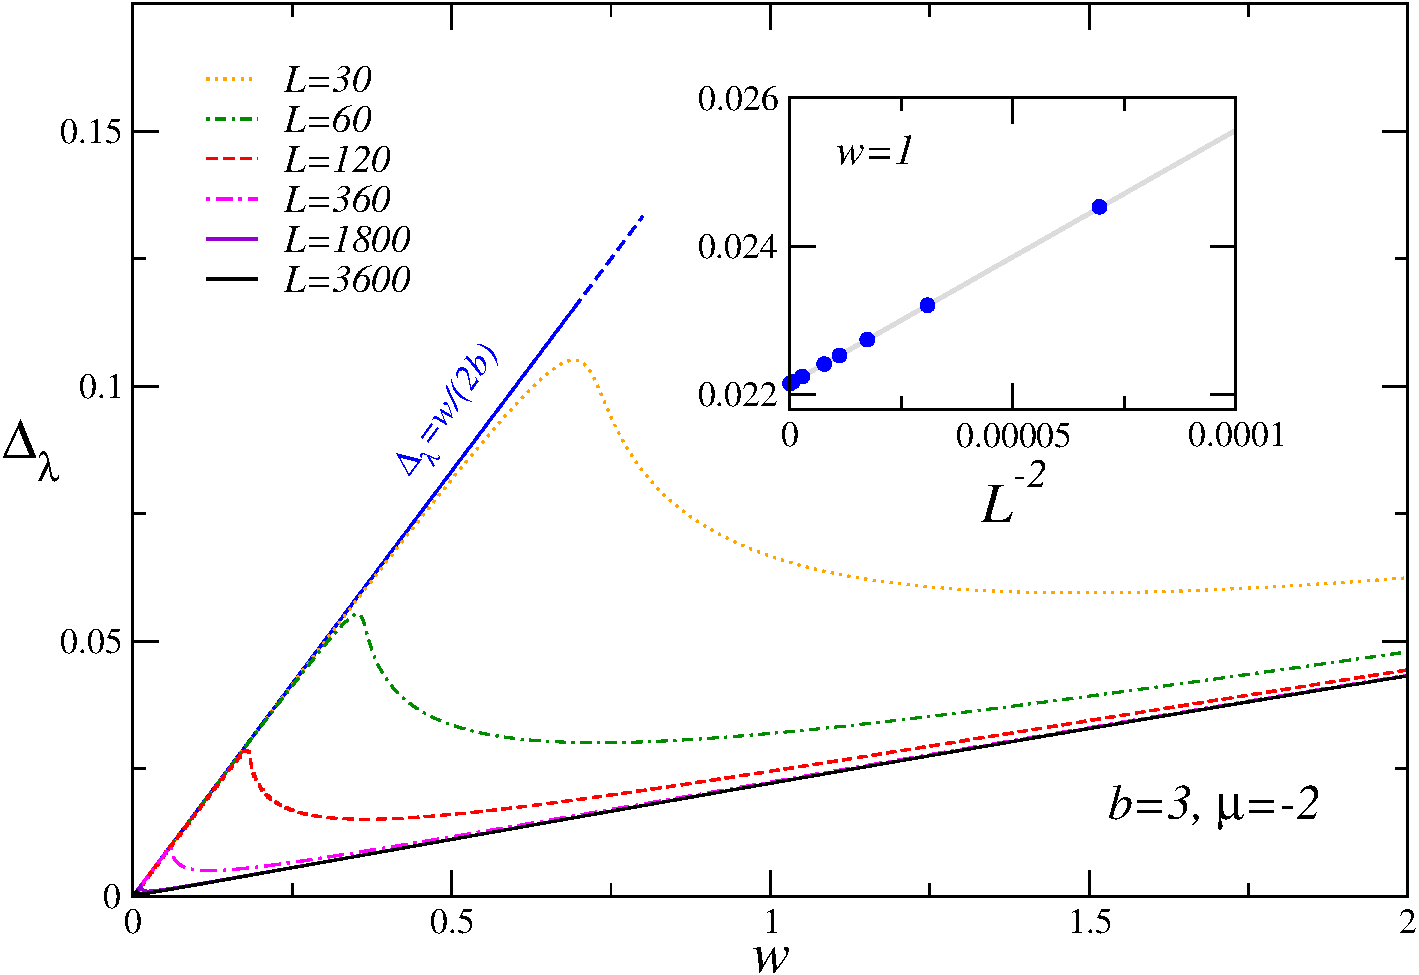
\includegraphics[width=6.4cm]{imm/gapliouv3b.pdf}
	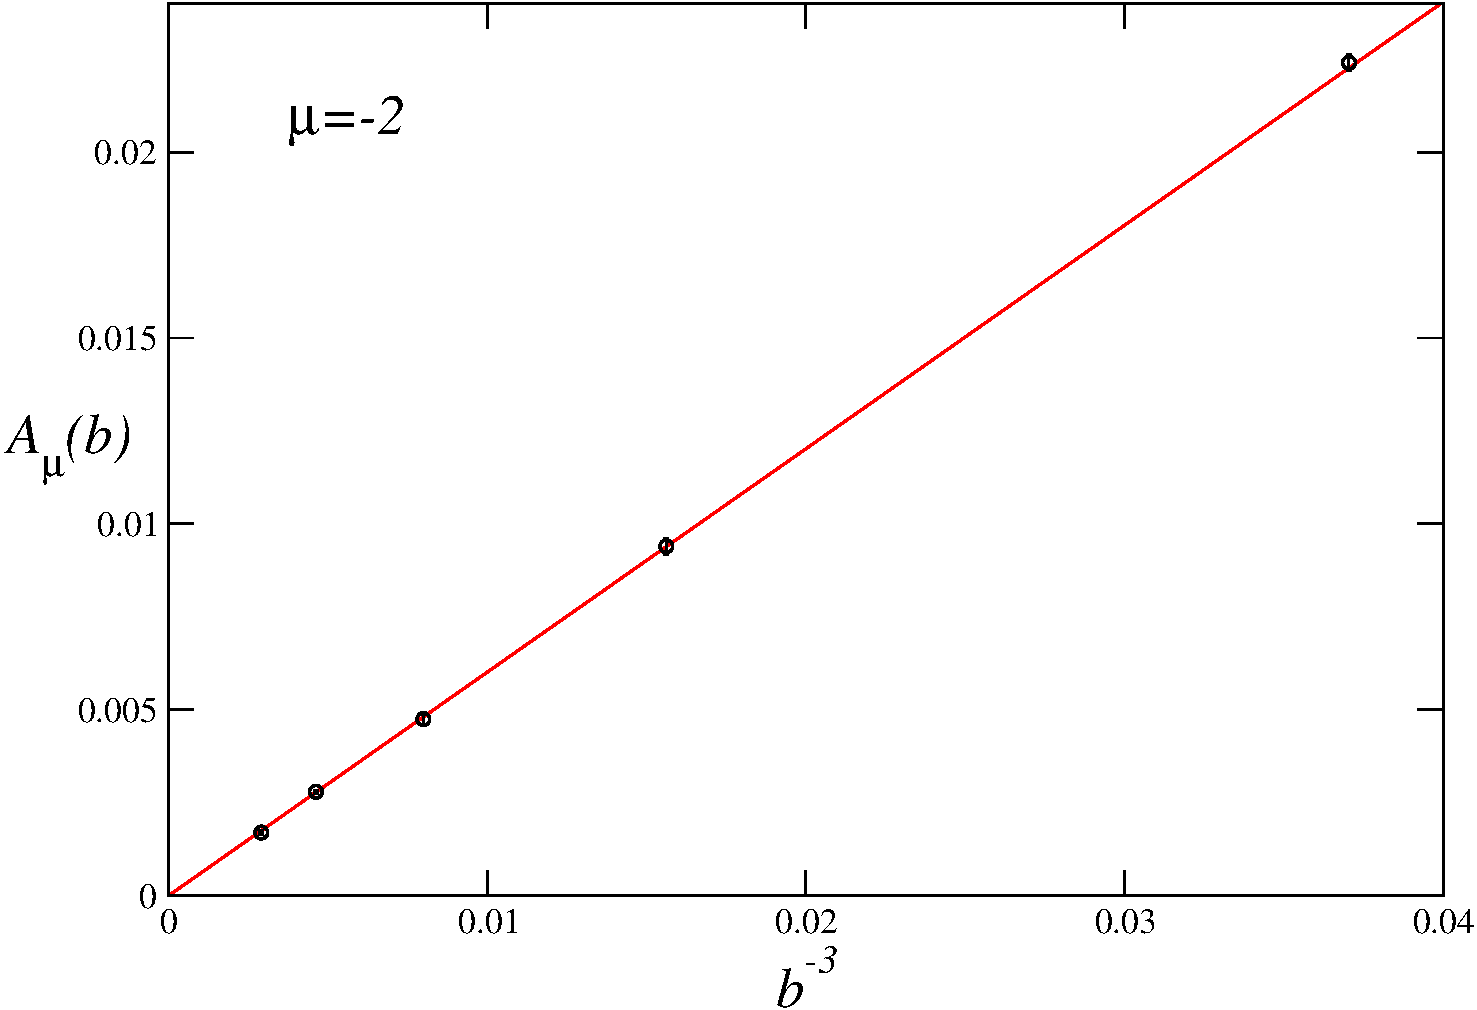
\includegraphics[width=6.4cm]{imm/ratelatetime.pdf}
    \caption{Liouvillian gap $\Delta_\lambda$ in terms of the dissipation coupling $w$ for $b=3$ and fixed $\mu=-2$.}
    \label{fig_liouvgap3b}
\end{figure}
\begin{equation}
    \Delta_\lambda(w, b)=A_\mu(b) w\,,\quad A_\mu(b)=\frac{C_\mu}{b^{3}}\,,\quad w>w_*\,,
    \label{eq_liouvillian_gap_largeL}
\end{equation}
\end{frame}

\begin{frame}
	\frametitle{Liouvillian gap $b$ fixed}
\begin{figure}
    \centering
    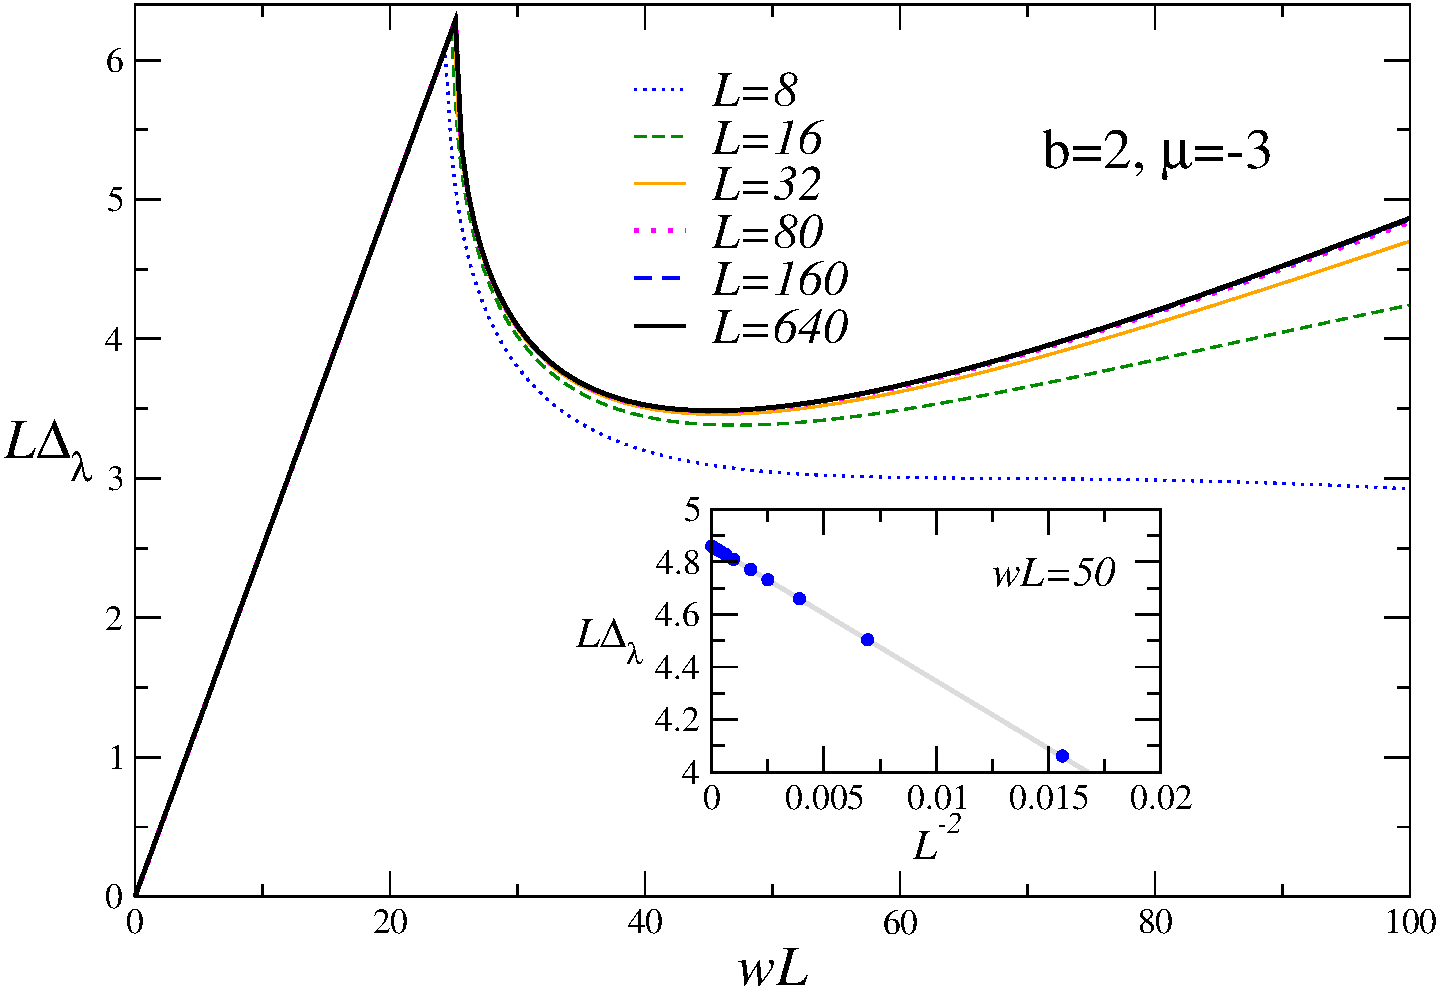
\includegraphics[width=8cm]{imm/scalingDeltaapbc.pdf}
    \label{fig_ratelatetime}
\end{figure}

\end{frame}

\begin{frame}
	\frametitle{Liouvillian gap $n$ fixed}
\begin{figure}[!b]
    \centering
    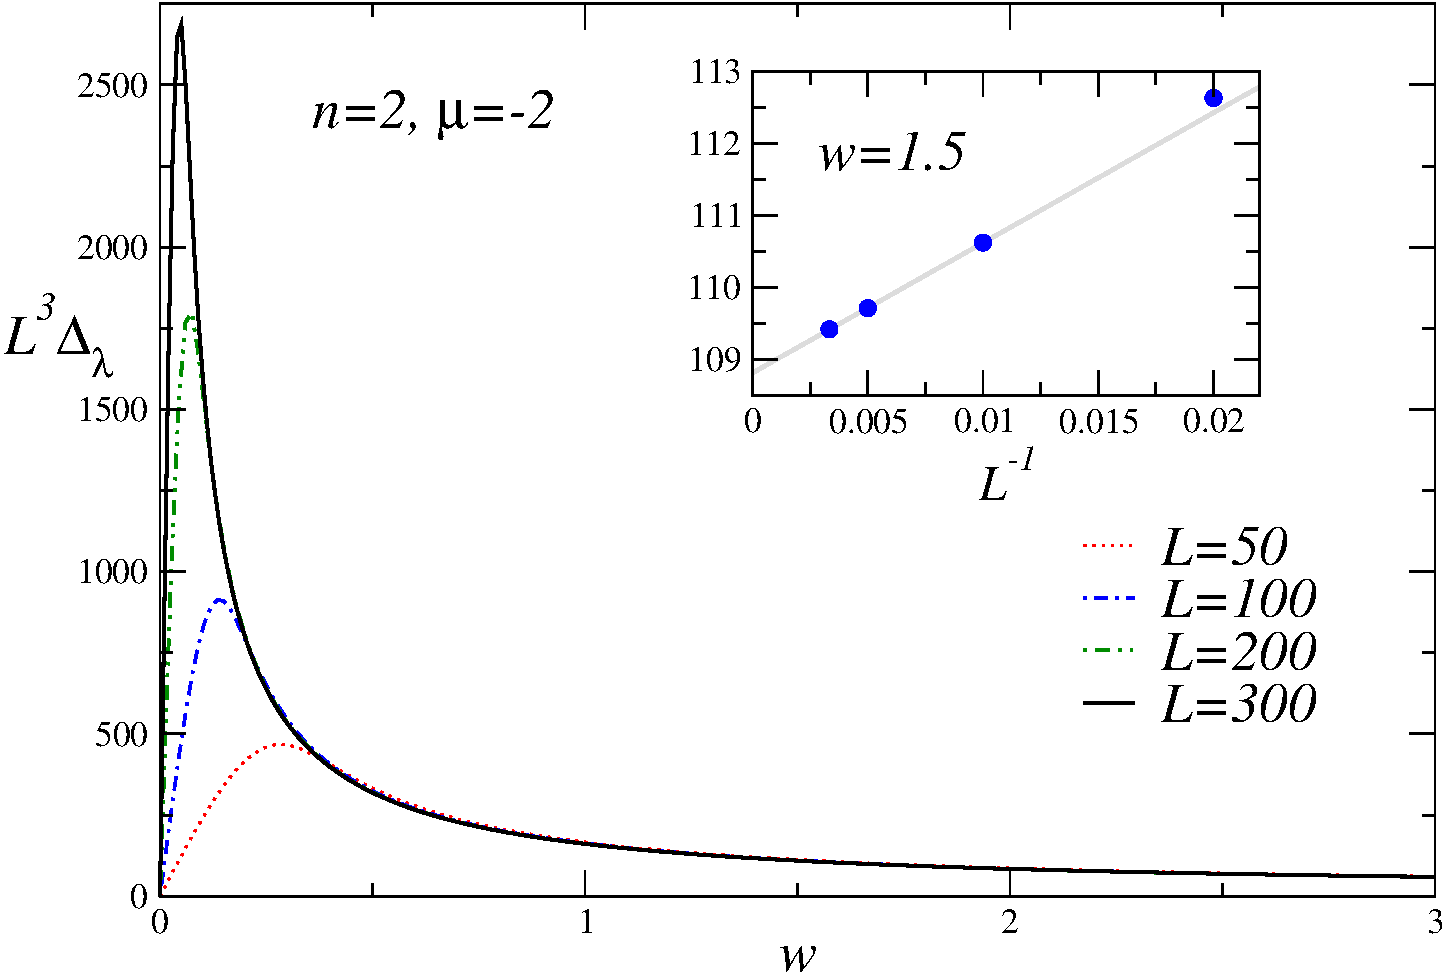
\includegraphics[width=6.4cm]{imm/delantipk0bl2L3Dw.pdf}
    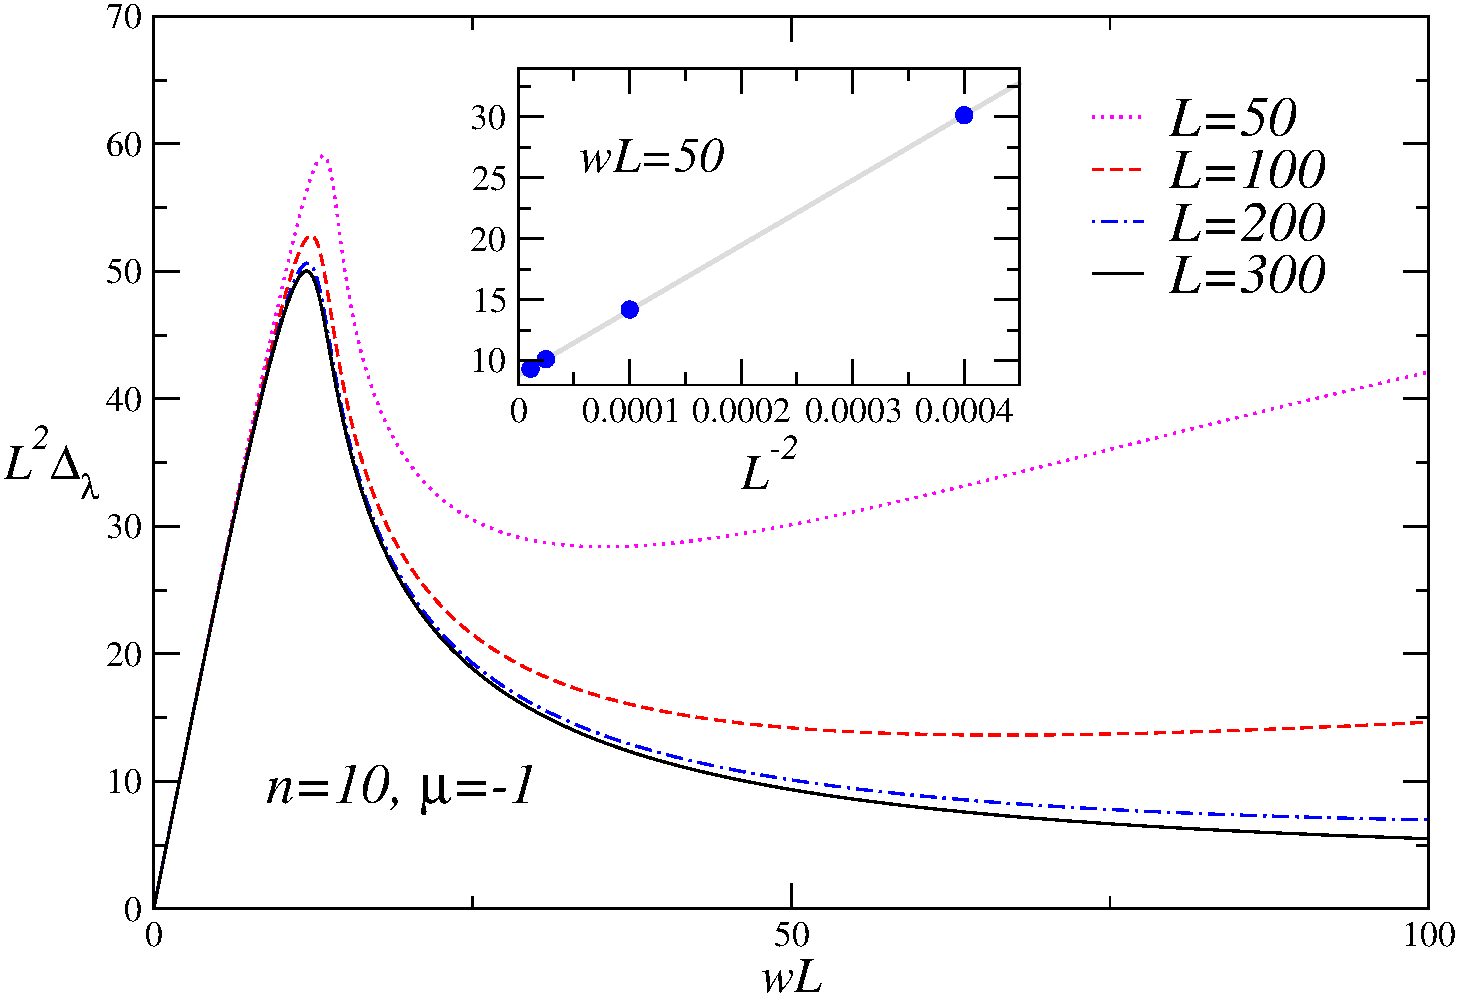
\includegraphics[width=6.4cm]{imm/scalingDeltanfixedmuminus1.pdf}
	\label{fig_scaling_delta_apbc}
\end{figure}

\end{frame}

\begin{frame}
	\frametitle{Dynamic Finite Size Scaling}
	The correlation function as observable:
	\begin{align}
        C(x, y, t)&\equiv{\rm Tr}[\rho(t)(\hat{c}^\dagger_x\hat{c}_y+\hat{c}^\dagger_y\hat{c}_x)]\,,\\
        P(x, y, t)&\equiv{\rm Tr}[\rho(t)(\hat{c}^\dagger_x\hat{c}^\dagger_y+\hat{c}_y\hat{c}_x)]\,.
    \label{eq_def_two_point_functions_C_P}
	\end{align}


	The scaling parameters are set:
	\ba{}
	M_{i/f}=(\mu_{i/f}-\mu_c)L^{y_\mu} &\qquad y_\mu = 1 \pc \\
	\Theta = t L^{-z}\,,\,\, z=1 \,\, 
	{\rm for} \,\, t \sim L &\pc \qquad
	\Theta = t /\Delta_\lambda \,\, 
	{\rm for} \,\, t\sim L^3 \pc \\
	\gamma_b=\frac{wL^{z}}{b}\,& \,\,.
	\ea


	The Scaling Laws can be expressed:
	\begin{align}
    C(x, y, t) &\approx L^{-2y_c}\mathcal{C}(M_i, M_f, \{X_i\}, \Theta, \gamma_b) \,\, ,   \notag \\
    P(x, y, t) &\approx L^{-2y_c}\mathcal{P}(M_i, M_f, \{X_i\}, \Theta, \gamma_b)\,.\notag
\end{align}

\end{frame}

\begin{frame}
	\frametitle{Numerical Results}
	\begin{figure}
    \centering
    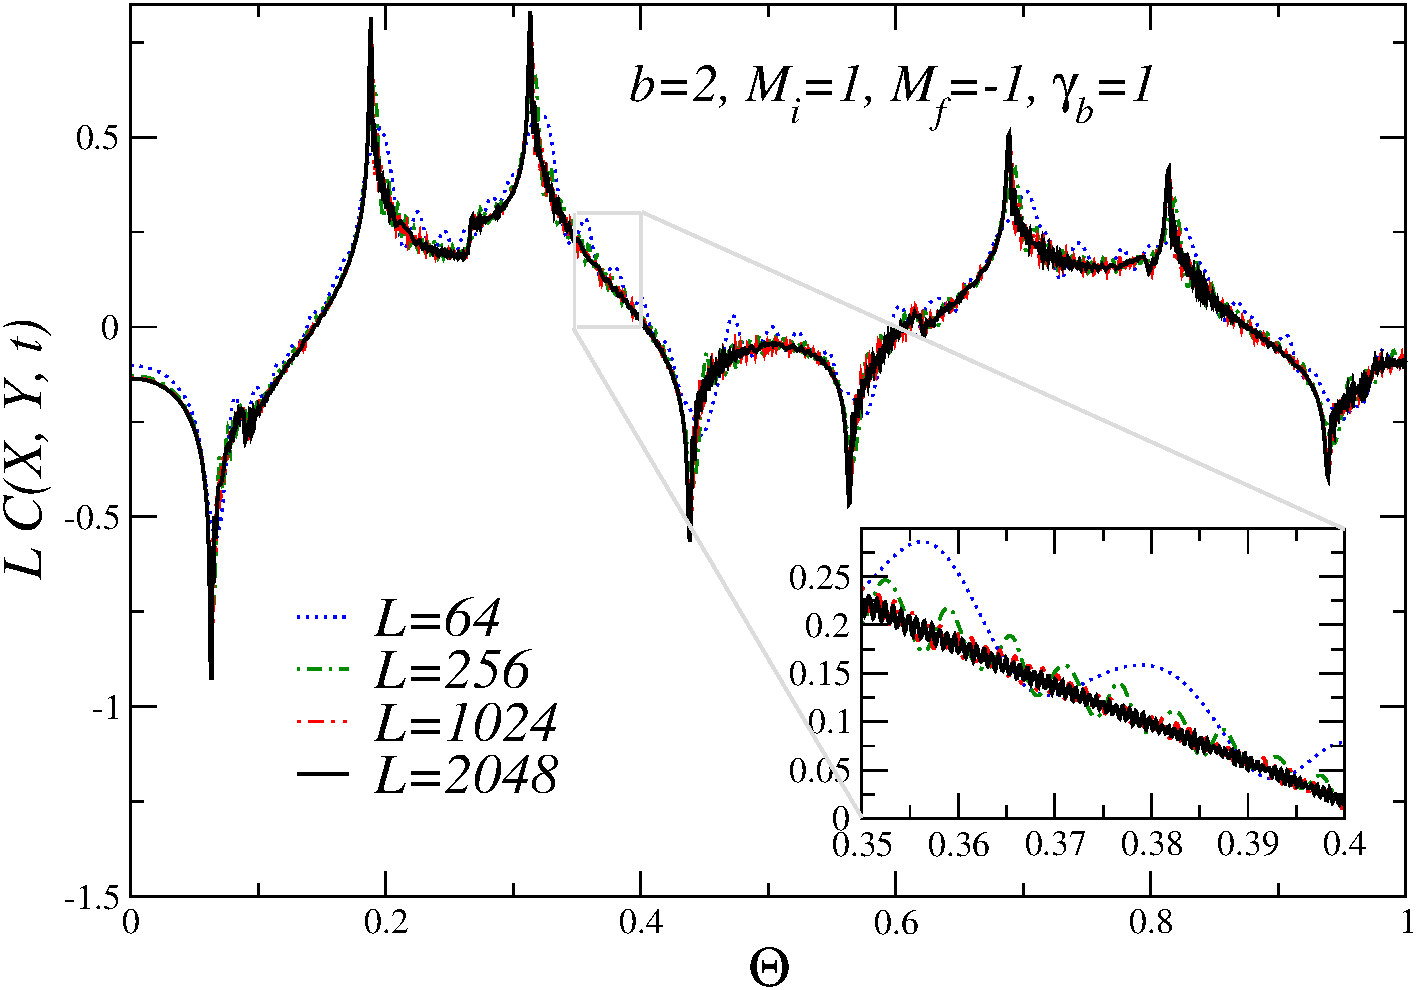
\includegraphics[width=6.4cm]{imm/Cscaling2b.pdf}
    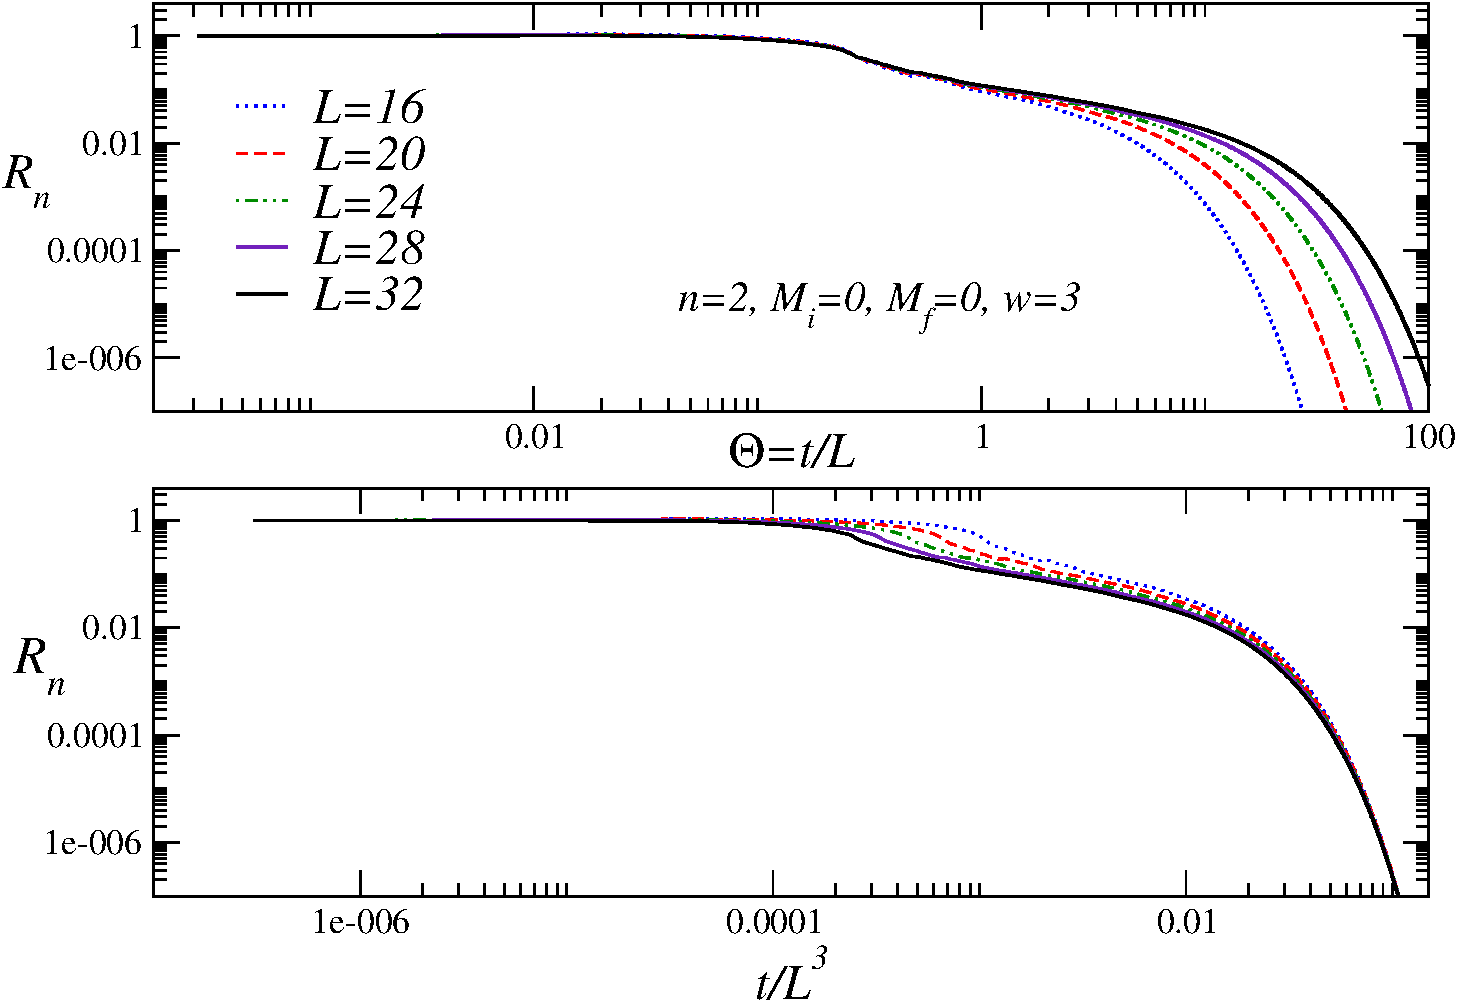
\includegraphics[width=6.4cm]{imm/fss_and_gap_n_fixed.pdf}
    \label{fig_Cscaling2b}
\end{figure}
We introduce the RG invariant quantity $R_n$ defined as 
\begin{equation}
    R_n = \frac{N(t) - N_{\text{asy}}}{N(0) - N_{\text{asy}}}\,,
    \label{def_Rn}
\end{equation}
where $N(t)=\sum_x^L\langle\hat c^\dagger_x \hat c_x(t)\rangle$
and $N_{\text{asy}}=\lim_{t\to\infty}N(t)$. 

\end{frame}
